% A snapshot of Lawrence Sullivan Ross' history.
%
% TODO FOR VERSION 2.0:
%   -   Research Texas succession statement, and Confederate constitution; what did 
%       LSR sign/acknowledge/fight for? 
%   -   Research Texas Constitutional Convention poll tax, LSR vote, and the resultant
%       arguments for and against sufferage restrictions. 
%   -   What constitutional committees did Ross serve on? 
%   -   LSR statement about serving all peoples regardless of color at Waco house
%   -   LSR and PVAMU 
%   -   LSR as governor, when state railcars were segregated.
%
% Good research locations:
%   -   Cornell University Library Civil War Documents. "The War of the Rebellion:
%       a Compilation of the Official Records of the Union and Confederate Armies."
%       URL: http://collections.library.cornell.edu/moa_new/waro.html
%
\documentclass[12pt]{article}
\usepackage[margin=1in]{geometry}
\usepackage{graphicx} %enable image embedding
\usepackage{longtable}
\usepackage{csquotes} %display quotes
\usepackage{url}

% bibliography
% basic information here: https://www.overleaf.com/learn/latex/biblatex_citation_styles
\usepackage[
    backend=bibtex,
    citestyle=numeric
]{biblatex}
\addbibresource{references}

% document misc: 
\parindent 0pt % no indents for new paragraphs
\renewcommand{\familydefault}{\sfdefault}

% table of contents:
\usepackage{color}
\usepackage{hyperref}
\hypersetup{
    colorlinks=true,
    linktoc=all,
    linkcolor=black,
}

% table row padding
{\renewcommand{\arraystretch}{1.5}

% -----------------------------------------------------
% Document start.
% -----------------------------------------------------
\begin{document}
\Large{\textbf{Lawrence Sullivan Ross \\}}
\large{Brief, incomplete answers to FAQ's on his treatment of African Americans \\}
\rule{\textwidth}{1pt}
\\John Rangel\\rangel.john.j@gmail.com\\15 June 2020
\section{Summary}
\parskip 2.0ex
Lawrence Sullivan Ross' campus statue and position within Texas A\&M's culture are the subject of spirited debate among current and former students. Attempted answers to several common questions raised in these discussions are presented. The questions discussed are subjective and focus on Lawrence Ross' documented behaviors, beliefs, and actions concerning African Americans before, during, and after the Civil War. 

Every effort was made to answer the included questions with publicly available historical resources. The presented information can be verified, expanded upon, or proven incorrect by any reader with a reliable internet connection. Answers contain citations for every statement, and almost every citation contains a URL. 

Interpretation of the presented historical resources is minimal, however the reader should be aware of the implicit bias present in any and every discussion over Lawrence Ross' past. Likely bias sources in this document include the author's affiliation with Texas A\&M, the author's personal and cultural experiences, and limited access to research materials because of COVID-19-related institutional closures.

This document was prepared by a spirited Aggie with no professional background in history or  historical research. It should serve as a conversation aide or stepping stone for further research. Better, more comprehensive historical sources that improve or reject the offered answers likely exist. 

% table of contents:
\parskip 0.5ex
\newpage
\tableofcontents
\parskip 2.0ex

% -----------------------------------------------------
% Purpose and scope.
% -----------------------------------------------------
\newpage
\section{Document purpose and scope}
This document is meant to provide a historical framework for discussions on Lawrence Sullivan Ross' place in Texas A\&M's culture. These discussions were prompted by the 2020 United States cultural reckoning in the wake of George Floyd's death at the hands of Minnesota police officers. 

This document attempts to answer common questions about Lawrence Ross' behaviors, beliefs, and actions concerning African Americans before, during, and after the Civil War. This document does not discuss Lawrence Ross' history with Native Americans, his years as president of the Agricultural and Mechanical College of Texas, or what role he should play in Texas A\&M's current and future culture. 

% -----------------------------------------------------
% Timeline.
% -----------------------------------------------------
\newpage
\section{Timeline of notable events}
A timeline of arbitrary state and national events is presented with a timeline of Lawrence Ross' personal and family events. 

% This file was autogenerated by timeline.py.
%
\begin{longtable}{|p{0.06\linewidth}|p{0.4\linewidth}|p{0.4\linewidth}|p{0.1\linewidth}|} 
\caption{High level timeline of Lawrence Ross' family and personal life.} \\ 
\hline 
\textbf{Year} & \textbf{State or national history} & \textbf{LSR personal or family history} & \textbf{Source} \\ 
\hline 
1835 & Texas revolution begins 
(October 2, 1835) &   &   \\ 
\hline 
1836 & The Battle of the Alamo 
(February 23 through March 6, 1836) &   &   \\ 
\hline 
1836 & Texas Declaration of Independence is adopted (March 2, 1836) &   &   \\ 
\hline 
1838 &   & LSR is born to Shapley Ross and Catherine Fulkerson in Iowa (September 27, 1838) & \cite{rosspapersummary} \\ 
\hline 
1838 &   & Shapley Ross runs to Texas after physical altercation with a lawyer over a runaway slave (sometime in 1838). Catherine Fulkerson follows with rest of family shortly after.  & \cite[pg. 53]{page} \\ 
\hline 
1845 & Texas is annexed into the United States as the 28th state in the Union (December 29, 1845) &   &   \\ 
\hline 
1849 &   & Ross family moves to Waco permanently (1849) & \cite{rosspapersummary} \\ 
\hline 
1859 &   & LSR graduates from Wesleyan University in Alabama (1859) & \cite{rosspapersummary} \\ 
\hline 
1861 &   & LSR resigns from active duty Texas Ranger service (1861; immediately before U.S. Civil War begins, but no date given) & \cite{rosspapersummary} \\ 
\hline 
1861 & United States Civil War begins (April 12, 1861) &   &   \\ 
\hline 
1861 &   & LSR marries Elizabeth Dorothy Tinsley (May 28, 1861) & \cite{rosspapersummary} \\ 
\hline 
1861 &   & Private LSR elected Major in the 6th Regiment of Texas Cavalry by his peers & \cite[pg. 36 and 37]{texasbrigade} \\ 
\hline 
1862 & Battle of Antietam (September 17, 1862). Bloodiest day in US military history with 22,717 dead, wounded, or missing. &   &   \\ 
\hline 
1863 & Emancipation Proclamation issued by President Abraham Lincoln (January 1, 1863) &   &   \\ 
\hline 
1863 & Battle of Gettysburg (July 1 thru 3, 1863) &   &   \\ 
\hline 
1863 &   & LSR promoted to Brigadier General (December 1863). Ross was 25 years of age. Ross commanded a cavalry brigade in the Army of Tennessee. & \cite{rosspapersummary} \\ 
\hline 
1865 & United States Civil War ends (April 9, 1865) &   &   \\ 
\hline 
1865 & President Abraham Lincoln is shot by John Wilkes Booth (April 14, 1865) and dies shortly after (April 15, 1865) &   &   \\ 
\hline 
1865 & Union general Gordon Granger reads ‘General Order No. 3’ to the public in Galvaston, TX, announcing total emancipation of those held as slaves (June 18, 1865; commonly known as Juneteenth) &   &   \\ 
\hline 
1865 & 13th Amendment to the US Constitution is adopted, formally abolishing slavery (December 18, 1865) &   &   \\ 
\hline 
1873 &   & LSR elected sheriff of McLennan County, Texas (1873) & \cite{rosspapersummary} \\ 
\hline 
1876 &   & LSR attends the Texas Constitutional Convention as a delegate from Central Texas (1876) & \cite{rosspapersummary} \\ 
\hline 
1880 &   & LSR elected Texas state senator, going on to serve one term (1880) & \cite{rosspapersummary} \\ 
\hline 
1887 &   & LSR becomes Governor of Texas (January 18, 1887). Ross would go on to serve two terms as governor, leaving office January 20, 1891.  & \cite{tsl} \\ 
\hline 
1889 &   & Shapley Ross, father to LSR, dies (September 17, 1889) & \cite{rosspapersummary} \\ 
\hline 
1891 &   & LSR leaves the office of the Governor of the State of Texas (January 20, 1891 & \cite{tsl} \\ 
\hline 
1891 &   & LSR accepts position as President of the Agricultural and Mechanical College of Texas (1891) & \cite{rosspapersummary} \\ 
\hline 
1898 &   & LSR dies at home (January 3, 1898). Ross was still college president at the time.  & \cite{rosspapersummary} \\ 
\hline 
\end{longtable}

% -----------------------------------------------------
% Pre Civil War frequently asked questions.
% -----------------------------------------------------
\newpage
\section{Pre Civil War FAQ's and attempts to answer them}

% Thoughts on slavery before civil war?
\subsection{What were LSR's thoughts on slavery before the Civil War? }
Preliminary research found little evidence on Lawrence Ross' opinion on slavery before the Civil War. Vaughan searched some of Lawrence Ross' correspondence archived at the Baylor University Library's Ross Collection and found no explicit statements on Lawrence Ross' ideas or practices regarding slavery \cite{vaughan:email}. Lawrence Ross made no mention of his stance on slavery in the online and published correspondence between Lawrence Ross, his wife Elizabeth Ross, and other relatives or friends viewed by the author. 

% Did LSR or family ever own slaves?
\newpage
\subsection{Did LSR or his family ever own slaves? }
Preliminary research found no evidence that Lawrence Ross ever owned, traded, or sold slaves. According to Page, the 1860 McLennan County Slave Census, and the 1862, 1863, and 1864 McLennan County Tax Rolls, do not list Lawrence Ross as a slave owner \cite[pg.49]{page}.

Preliminary research found evidence that Lawrence Ross' parents owned slaves. According to Page \cite[pg.49]{page}, the 1830 Lincoln County, MO Census lists Shapley Ross, Lawrence Ross' father, with Shapley Ross' mother and several slaves. Page lists several historical sources that state Shapley Ross first came to Texas after a physical altercation with a lawyer over a runaway slave made him flee the local authorities \cite[pg.50--51]{page}. 

Lawrence Ross was born September 27, 1838. Page found evidence that Shapley Ross owned several slaves between 1840 and the late 1860's, however the number varies with time \cite[pg.51--55]{page}. 

The author finds it reasonable to presume the Ross family owned at least one slave, and likely several, at points throughout Lawrence Ross' childhood and teenage years. Lawrence Ross' treatment of these slaves as a child, teenager, and young adult would make fascinating research. 

% -----------------------------------------------------
% Civil War Frequently asked questions.
% -----------------------------------------------------
\newpage
\section{Civil War FAQ's and attempts to answer them}

% why did LSR fight in the civil war?
\subsection{Why did LSR fight for the Confederate States of America?}
Preliminary research suggests Lawrence Ross' motivation for Confederate service was driven by his loyalty to the state of Texas. Lawrence Ross wrote he would resign his Confederate army position and return to defend Texas if the state was ever directly threatened and the Confederate army did not order the Texas regiment back. 
\begin{displayquote}
A rumor has just reached us that has created much excitement, It is to the effect that several war vessels have appeared off Galveston (Texas), and demanded the women and children to be sent from the City. If this prove correct and my Regiment is not ordered back I will resign and return. 

-- Ross to his wife Lizzie Ross, October 5, 1861 \cite[pg. 9]{sullyletters}
\end{displayquote}

Several of Lawrence Ross' letters to his wife, Elizabeth Ross, describe a sense of duty as his reason for military service.
\begin{displayquote}
I must confess that I desire to return. Yet I feel that my duty to my Country demands the course I am pursuing, and hence becomes more tolerable. 

-- Ross to his wife Lizzie Ross, September 7, 1861 \cite[pg. 3]{sullyletters}
\end{displayquote}

The wording and tone of Lawrence Ross' personal Civil War letters suggest this "sense of duty" stemmed from a perceived aggression by the U.S. government on Texas, and the Southern states in general. Lawrence Ross refers to his "Country" as "(struggling) for life beneath a crushing weight of oppression" \cite[pg. 28]{sullyletters}, and various Southern military units determined to "never bend the suppliant knee to a Tyrants Sway" \cite[pg. 17]{sullyletters}. In one letter Lawrence Ross described federal activity in Missisippi as "Abraham Lincoln's conquest" \cite[pg. 54]{sullyletters}.

At an October 1892 speech to Confederate Army veterans recorded in the Galvaston Daily News, Lawrence Ross said slavery was not a primary motivator for the "great majority of Confederates":
\begin{displayquote}
“In behalf of thousands of old Confederates I want to record the fact today, that while slavery was undoubtedly an element which served to keep the public mind of the country like an angry sea that was continually casting up mire and dirt, it did not represent the principles for which the great majority of Confederates contended.  As an evidence of this fact I simply illustrate a general truth by saying that not 100 of the 1200 men composing the regiment in which I enlisted at the commencement of the struggle ever owned or expected to own a slave.  Very many of them had not left their former northern homes long enough to entitle them to vote here and yet when their adopted state took the fatal step, though subjected to the severest ordeal through which men wore ever called upon to pass, they determined to share her fate and they adhered to her cause with consistent and unshaken fidelity until it perished by war.” 

-- Lawrence Sullivan Ross, at an October 26, 1892 Confederate Army veterans reunion held at the State Fair \cite{gdaily:1892-10-26}.
\end{displayquote}

Page reasons however that whatever Lawrence Ross' motivations for Confederate army service were, Lawrence Ross must have known that he was supporting a government dedicated to the preservation of slavery \cite[pg. 59]{page}. Taken without context and without correspondence not yet found by the author, Lawrence Ross' personal letters suggest Lawrence Ross was at the very least dedicated to the Texas government as it existed in rebellion. The Texas declaration of secession explicitly stated slavery as a primary reason for leaving the Union.
\begin{displayquote}
We hold as undeniable truths that the governments of the various States, and of the confederacy itself, were established exclusively by the white race, for themselves and their posterity; that the African race had no agency in their establishment; that they were rightfully held and regarded as an inferior and dependent race, and in that condition only could their existence in this country be rendered beneficial or tolerable.

-- A declaration of the causes which impel the State of Texas to secede from the Union \cite{tx:secede}
\end{displayquote}

The 1861 Constitution of Texas likewise explicitly supported slavery.
\begin{displayquote}
ARTICLE VIII: Slaves.

SEC. 1. The Legislature shall have no power to pass laws for the emancipation of slaves.

SEC. 2. No citizen, or other person residing in this State, shall have power by deed, or will, to take effect in this State, or out of it, in any manner whatsoever, directly or indirectly, to emancipate his slave or slaves.

SEC. 3. The Legislature shall have no power to pass any law to prevent immigrants to this State, from bringing with them such persons of the negro race as are deemed slaves by the laws of any of the Confederate States of America; provided, that slaves who have committed any felony may be excluded from this State.

-- Article VIII sections 1,2, and 3 of the 1861 Texas Constitution \cite{tx:1861constitution}. Sections 4,5, and 6 excluded for brevity.
\end{displayquote}

% army service?
\newpage
\subsection{What was LSR's Confederate Army service?}
Lawrence Ross enlisted as a private in a cavalry company commanded by his older brother, Peter F. Ross \cite{rosspapersummary}. Lawrence Ross was elected by his peers to Major in the 6th Regiment of Texas Cavalry sometime in 1861 \cite[pg. 36--37]{texasbrigade}. Lawrence Ross was promoted to his highest Confederate Army rank -- Brigadiar General of an Army of Tennesee cavalry brigade -- in December 1863 \cite{rosspapersummary}. Lawrence Ross was 25 years old at the time. Lawrence Ross saw combat many times, however his combat record is outside the scope of this document. 

% attitude towards african americans during the civil war? 
\newpage
\subsection{How did LSR view and treat African Americans during the Civil War?}
A survey of Lawrence Ross' personal Civil War correspondence revealed two instances where Lawrence Ross negatively referred to African Americans. Lawrence Ross expressed frustration with the overall state of the Confederacy in Arkansas and Missouri in the Civil War's first year. Among frustrations over disease and poor winter clothing provisions, Lawrence Ross wrote about his first impressions of the Missourians' dedication to the Confederacy and disparaged the slaves in the state \cite[pg. 13-14]{sullyletters}.
\begin{displayquote}
More than one half of them are Abolitionists at heart and in sentiment, and the Majority of the other half are rendering Lincoln good service by running off to Texas or by their unwillingness to contribute a single article to alleviate the sufferings of the Confederates...They are sold to Lincoln -- "Joined to their idol" and should be let alone -- and may the lot of the degraded slave -- unworthy the boon of Equality -- freedom, or National respect, go with them as their portion.

-- Lawrence Ross to Elizabeth Ross, October 14, 1861 \cite[pg. 14]{sullyletters} 

\end{displayquote} 

Lawrence Ross again expressed frustration at the Confederacy's inability to keep its soldiers properly dressed when he described the ludicrous outfit one of his cousins was forced to wear for lack of better clothing as something "no Negro in Waco" would even wear.
\begin{displayquote}
Here in this condition I met Willie Wallace, my cousin, a Young man that has been raised in affluence and luxury, and possessing almost foppish pride in dress, and in all things as particular as any Old Maid, and around his shoulders he had thrown an old cloak that hung in ribbons and tags, covered with dust and slick with grease, and this together with an old pair of pants, that perhaps no Negro in Waco could be induced to wear, constituted the sum total of his wardobe -- And in this condition has he been marching from point to post, and in Every Battle in the State since the war began.

-- Lawrence Ross to Elizabeth Ross, October 28, 1861 \cite[pg. 16]{sullyletters}
\end{displayquote}

Preliminary research found one negative example of Lawrence Ross' military treatment towards African Americans. Page describes an instance during the Civil War where Lawrence Ross refused to recognize African American Union soldiers as soldiers during surrender negotiations with a Union officer:
\begin{displayquote}
Brigadier General L. S. Ross cut off and surrounded the Federal garrison at Yazoo City, Mississippi in March, 1864, and, on the fifth, demanded its surrender.  “We squabbled about the terms of the capitulation,” reported the General, “as I would not recognize Negroes as soldiers, or guarantee them nor their officers protection as such.”

-- William Page, quoting "Negro Casualties in the Civil War" \cite[pg. 62]{page}.
\end{displayquote}

Context may provide some relief to history's judgement on Lawrence Ross for this episode. Two soldiers under Ross' command were murdered after surrendering earlier during the fighting around Yazoo City:
\begin{displayquote}
During the operations on the Yazoo, two young men of the Sixth Texas were brutally murdered by the enemy, after surrender; and thus was inaugurated an informal "war to the knife," which claimed many victims who otherwise would only have experienced the rigors of captivity. 

-- "Ross' Texas Brigade," paragraphs and footnote on page 105 \cite[pg. 105]{texasbrigade}.
\end{displayquote}

Page quotes "The Lone Star Defenders: a Chronicle of the Third Texas Cavalry, Ross Brigade" to describe the same events with more detail:
\begin{displayquote}
The enemy [Union soldiers] had the advantage of several redoubts and riflepits, the main central redoubt being situated on the plank road leading from Benton to Yazoo City.  We fought them nearly all day, and at times the fighting was terrific.  With the Third Texas in advance we drove in their pickets and took possession of all the redoubts but the larger central one.  This one was in command of Major George C. McKee, of the Eleventh Illinois Regiment with nine companies...[including] Major Cook, with part of his First Mississippi Negro cavalry, the same that had murdered the two Sixth Texas men...at four o'clock in the afternoon we had it entirely surrounded, we being in front some 150 yards distant. At this juncture General Ross sent Major McKee a flag of truce and demanded an unconditional surrender. The firing ceased and the matter was parleyed over for some time. The first message was verbal, and Major McKee declined to receive it unless it was in writing. It was then sent in writing, and from the movements we could see, we thought they were preparing to surrender. But they refused, owing perhaps to the fact that General Ross declined to recognize the Negro troops as soldiers; and how they would have fared at the hands of an incensed brigade of Texas troops after they had murdered two of our men in cold blood was not pleasant to contemplate. As for the Negro troops, -- well, for some time the fighting was under the black flag -- no quarter being asked or given.  Retaliation is one of the horrors of war, when the innocent are often sacrificed for the inhuman crimes of the mean and bloodthirsty.

-- "The Lone Star Defenders: a Chronicle of the Third Texas Cavalry, Ross Brigade", quoted by Page \cite[pg. 61--62]{page}.
\end{displayquote}

Lawrence Ross' decision on black Union Prisoners of War (POW's) at the Yazoo City conflict, and whether Lawrence Ross' commonly made the same decision about black POW's at other engagements, should be further investigated. Black Union soldiers faced prejudice from within the Union army and as Confederate POW's \cite{natarch:pow}. The Confederacy's treatment of captured black Union soldiers is a topic far beyond this document's scope however. The reader is encouraged to perform their own research. 

% -----------------------------------------------------
% Post Civil War Frequently asked questions.
% -----------------------------------------------------
\newpage
\section{Post Civil War FAQ's and attempts to answer them}

% thoughts on slavery after civil war?
\subsection{What were LSR's thoughts on slavery after the Civil War?}
Several sources suggest Lawrence Ross considered slavery a dead part of the South that should never return. Lawrence Ross wrote in his post Civil War presidential pardon request that:

\begin{displayquote}
He would further say that he regards the slavery question as finally settled, and would view any attempt to reestablish slavery in the South as injudicious \& impolitic.  He believes that the People of the South should regard the question as settled for ever, and that it devolves upon the Southern States in their respective conventions to so provide in their organic laws.

-- L.S. Ross application for special pardon to the President of the United States, August 4, 1865 \cite{pardonrequest}.
\end{displayquote}

Page lists several speeches and documents where Lawrence Ross said the South's future lay in continued reunification with the North and adherence to the Union's federal laws and government \cite[pg. 161--167]{page}. A speech Lawrence Ross made to the annual reunion of Hood's Brigade said:

\begin{displayquote}
It is a remarkable fact that those who bore the brunt of battle were the first to forget old animosities and consign to oblivion obsolete issues.  They saw that nothing but sorrow and shame and the loss of the respect of the world was to be gained by perpetuating the bitterness of past strife.  And impelled by a spirit of patriotism they were willing by all possible methods to create and give utterance to a public sentiment which would best conserve our common institutions and restore that fraternal concord in which the war of the revolution left us and the Federal constitution found us.

-- Lawrence Ross' Address to the Annual reunion of Hood's Brigade, as recorded in the June 28, 1887 The Fort Worth Daily Gazette \cite{fwg:1887-06-28}.
\end{displayquote}

% attitude towards african americans after civil war? 
\newpage
\subsection{How did LSR treat African Americans in his various public offices?}
Preliminary research revealed many examples where Lawrence Ross treated the African American community with equality and without prejudice during his various roles in public office. 

Lawrence Ross was nominated as the Texas Democratic Party's gubernatorial candidate in 1886 \cite[pg. 150-159]{benner:sulross}. Lawrence Ross returned to Waco, Texas after his nomination, where he was greeted by a large crowd of supporters. Lawrence Ross thanked the crowd for their support and pledged to enter office prepared to serve all Texans regardless of their party affiliation, race, or color.
\begin{displayquote}
(He) pledged himself to an honest, faithful and economic discharge of his duty, that he had used no money nor purchased no man's influence by promises or otherwise to secure the nomination he had received, he would go into office untrammeled and prepared to serve the whole people alike regardless of party affiliation or partisanship or color.

-- Ross Family Papers Box 2, folder 27 \cite{rosspapers}
\end{displayquote}

Lawrence Ross' terms as Texas governor were filled with racial violence between white and black citizens. An example provided by Page that stands out involved the murder of seven African Americans by white men jealous of their farmland:
\begin{displayquote}
In Wharton county is a village called Spanish Camp [where] some Negroes had gained possession of some land which they were quietly tilling and from which they had raised a crop. Some white men coveted the ground and ordered the Negroes to vacate.  This they refused to do. The matter came to a trial in a court of justice and the Negroes won the suit, the court sustaining their legal claim to the property...Finding that threats could not intimidate, nor law dispossess those colored men, their white antagonists, in the dead of night gathered a posse of their own diabolical breed, who armed themselves with Winchesters and shotguns, surrounded the house while eight Negroes were asleep inside, saturated the outside of the building with kerosene, while the inmates to whom the law had given possession were within, fired it, and as the roasting victims attempted to escape shot them down in cold blood, killing seven out of the eight and wounding the solo survivor.

-- San Marcos Free Press, 15 March 1888 \cite{sanmarcospress}.
\end{displayquote}

The Spanish Camp massacre came shortly after a white man named Thomas Forsyth was lynched by a mob after he murdered another man. Lawrence Ross, who issued a strong condemnation of Forsyth's lynching, was critized in the same article for not responding to the Spanish Camp massacre immediately in the same way \cite[pg. 97--98]{page}. It is not clear whether the article's criticism was well founded or editorialized however. Numerous examples of white-on-black atrocities that drew strong, public condemnation from Lawrence Ross are present in Page's document \cite[95--155, etc]{page}. 

Lawrence Ross dispatched a team of Texas Rangers to assist the local authorities with investigating and prosecuting the Spanish Camp massacre. Thirty-seven citizens of Wharton county, near Spanish Camp, protested the governor's action \cite[pg. 104--106]{page}. Lawrence Ross' response to the Wharton county protest letter, and his actions to handle subsequent lawlessness in Wharton county and Texas, became flashpoints in the contemporary racial tensions that gripped the state:
\begin{displayquote}
I have the honor to acknowledge the receipt of your protest against the presence of rangers in your county, and in reply I beg to say that I am unable to appreciate the force of your objections...the first invocation which I took upon my lips when assuming the functions of the executive office, was to maintain the constitution, and it enjoins upon me to see that the laws are faithfully executed, and a state denies protection to the citizen by ineffectually not executing as not by not making laws. Its expensive machine becomes a mockery when no security is furnished; when laws are made only to be trampled on; when crime stalks abroad unchallenged and unchecked; when the home is no longer a protection, but its sanctity is violated with impunity and shooting its unarmed inmates...

-- excerpt from L.S. Ross' response to Wharton county citizens \cite{gdaily:1888-03-21}.
\end{displayquote} 

Page quotes several subsequent newspaper articles, including those in the black press, that praised Lawrence Ross' response \cite[pg. 106--108]{page}:
\begin{displayquote}
The Spanish camp butchers will all be brought to justice, or The Gazette is sadly mistaken in Governor Ross. There will be protection for all people in Texas under Sul Ross, regardless of color, age, sex or previous condition of servitude. And this only is law, justice and liberty.

-- The Fort Worth Gazette, April 6, 1888 \cite{fwg:1888-04-06}
\end{displayquote}

Several days after the Spanish Camp massacre, two African Americans were murdered in Wharton county, prompting Lawrence Ross to send more Texas Rangers to the troubled area. Over 300 people protested Lawrence Ross' actions, but Lawrence Ross stated he would "send the whole militia of the State" if necessary:
\begin{displayquote}
...two Negroes were brutally murdered on Tuesday night in Wharton county, near the scene of a recent massacre of Negroes at Spanish Camp. This killing was on Battle’s plantation. Governor Ross sent a company of rangers to Wharton county to suppress lawlessness. Over 300 people protested, stating the feud would die out. Governor Ross being appealed to states that he will send the whole militia of the State if necessary to suppress the lawless element. 

-- Page, quoting the San Jose, CA Evening News \cite[pg. 101]{page} 
\end{displayquote}

Page provides many examples where Lawrence Ross intervened when local authorities struggled to investigate and prosecute these crimes, or where local authorities were forced to stand by while mobs lynched or executed both white and black suspects \cite[pg. 95--155, etc]{page}. These are not included in this report for brevity.

Page documents many examples of Lawrence Ross' equitable, respectful, or (arguably) friendly actions towards African Americans \cite{page}. Three examples are presented here for brevity.

Lawrence Ross was a pallbearer at the funeral of Armistead Ross, an African American and longtime servant to the Ross family:
\begin{displayquote}
Old Armistead Ross, one of the most hardworking, steady and wealthy colored men in Waco, was consigned to the earth yesterday...His funeral took place at 3 o’clock yesterday, and was attended by a large concourse of people, both white and black. The pall bearers who bore his coffin to the hearse were Gen. L. S. Ross, Sheriff W. T. Harris, County Clerk John W. Baker, Tom Padgitt, and John V. Smith. His remains were interred in the old cemetery.

-- The Waco Daily Examiner, 20 October 1883 \cite{wde:1883-10-20}.
\end{displayquote}

Lawrence Ross appointed William Holland the first superintendent of the Deaf, Dumb, and Blind Institute for Colored Youth. The author finds this appointment notable because William Holland was born into slavery in 1841. William Holland enlisted in the Union Army's 16th U.S. Colored Troops and saw combat in the battles of Nashville and Overton Hill \cite{tsha:willholland}. The author finds it reasonable to presume Lawrence Ross knew William Holland's history. The Austin Daily Statesman's obituary for William Holland suggests Lawrence Ross and William Holland had at the least a good professional relationship:

\begin{displayquote}
The superintendent of that institution [Deaf, Dumb, and Blind Institude for Colored Youth], when notified of his election, came before the governor and the board and told them that while he regarded their action as a great compliment he had some misgivings as to his ability to perform its duties with satisfaction to himself and to the state. The governor [Lawrence Ross] said to him: ‘I know you and have known of you for some years. If you can’t fill the place satisfactorily we can’t find a colored man in Texas who can. Try it.’

--Austin Daily Statesman, 21 June 1907 \cite{astatesman:1907-06-21}.
\end{displayquote}

Lawrence Ross as Governor pardoned or commuted the sentences of at least 31 African Americans \cite[pg. 146]{page}. Page cautions however that there is currently no way to compare Lawrence Ross' African American pardons and commuted sentencing record with other contemporary statesmen because the historical research on this topic is scarce \cite{page:email}.  

% -----------------------------------------------------
% Civil rights frequently asked questions.
% -----------------------------------------------------
\newpage
\section{Civil rights FAQ's and attempts to answer them}

% on poll taxes:
\subsection{Did LSR support a poll tax to disenfranchise African American voters?}
Lawrence Ross did not support -- and voted several times against -- a poll tax meant to disenfranchise African American voters during the Texas Constitutional Convention of 1875. 

Lawrence Ross was an elected delegate to the Texas Constitutional Convention of 1875. The proposed language of the 1876 Constitution's article on suffrage included payment of a poll tax as a necessary qualifier to vote "at all elections of the people held in this State" \cite[pg. 238]{tx:1876constitution:journ}. Lawrence Ross voted to amend the constitution's article on suffrage to no longer require payment of a poll tax. The amended section was adopted by a vote of 61 to 20 \cite[pg. 307-308]{tx:1876constitution:journ}. 

Several amendments were then introduced to put a poll tax requirement in different shapes and forms back into the constitution's suffrage article. Lawrence Ross voted each time with the majority to table these amendments \cite[pg. 308-310]{tx:1876constitution:journ}.

Lawrence Ross voted for language that would establish a poll tax as a revenue source to fund public education in the constitution's education article \cite[pg. 330-333]{tx:1876constitution:journ}. Payment of this poll tax would not be a prerequisite for suffrage however. 

% on segregation:
\newpage
\subsection{Did LSR support segregation?}

% Ku Klux Klan membership?
\newpage
\subsection{Was LSR a member of the Ku Klux Klan?}
There is no evidence that Lawrence Ross was a member of, or affiliated with, the Ku Klux Klan. Page writes on the subject that:

\begin{displayquote}
In recent years some people have claimed that Ross belonged to the Ku Klux Klan.  No evidence has been found that he belonged to the Klan during Reconstruction.  Ross’ attitudes and actions concerning mob violence while sheriff and governor are inconsistent with Klan membership.  Moreover, Ross could not have been a member of the Klan while governor or president of A\&M, because the Klan did not exist in Texas in the 1880s and 1890s.

An unfounded rumor concerning Sul Ross is that the Cushing Memorial Library at A\&M has his Klan robe.  This is not true.  The Cushing Library has three Klan robes in their collection.  They are marked with the names of J. F. Cavitt, M. C. Walker and one time Aggie football coach Dana X. Bible \cite[pg. 253]{page}.
\end{displayquote}

A preliminary search revealed no mention of the Ku Klux Klan in Lawrence Ross' correspondence archived at Baylor University's Sul Ross Collection \cite{vaughan:email}.

% -----------------------------------------------------
% Misc. asked questions.
% -----------------------------------------------------
\newpage
\section{Misc. FAQ's and attempts to answer them}

% contemporary black community thoughts?
\subsection{What did the black community think of LSR during his public positions after the Civil War?}
Preliminary research found many examples where the black community commended Lawrence Ross' actions as Governor of Texas. One example that stands out is the black community's support of Governor Ross' creation of "an asylum for the colored blind, deaf and dumb persons":

\begin{displayquote}
A delegation of colored citizens, consisting of Rev. A. Grant, J. J. Hamilton, Rev. Saml. Gates, Rev. C. H. Anderson and Prof. Blackshear, consulted Governor Ross yesterday upon matters of legislation appertaining to the interests of the colored people. The committee were favorably impressed with the governor’s views, as to the propriety of establishing an asylum for the colored blind, deaf and dumb persons, to be controlled by a board of colored men, as directors.

-- Austin Daily Statesman, 8 February 1887 \cite{astatesman:1887-02-08}.
\end{displayquote}

A letter from a "colored school teacher" commending Lawrence Ross' actions on the Spanish Camp massacre was published in the Austin Daily Statesman: 
\begin{displayquote}
Palestine, Texas, April 14, 1888

Dear Sir – Having noticed with great pleasure the firm and manly stand you have taken in sending rangers into Wharton county, to ferret out the perpetrators of that heinous crime committed upon the colored people of Spanish Camp, I am compelled to beg for forgiveness for sending you this as a token of my appreciation of your manliness and sterling worth of the chief executive of this state, and I express the sentiments of my people when I endorse and advocate your re-election as governor of this state.

Yours for True Manhood,

H. L. Price,
Teacher in Public Schools, Anderson County, Texas

-- Austin Daily Statesman, 17 April 1888 \cite{astatesman:1888-04-17}.
\end{displayquote}

A research area that deserves more attention is the black community's response to Lawrence Ross' death. Page again provides several examples \cite{page}, two of which are listed below. 

The first is a letter published in the Dallas Morning News "From a Colored Man" donating a dollar to the Ross monument fund:
\begin{displayquote}
From a Colored Man. \\
Austin, Tex., Feb. 17 – (To The News) – Inclosed find the sum of \$1, which you will add to the Ross monument fund.  The amount is small, but I hope it will do some good.  If every true and loyal Texan would do as much as we would be able to erect a monument that would be a credit to the name of our proud state and do honor to so grand a man as Gov. Ross.  Hoping the monument will meet with great success, I remain a true Texan, and believe in giving honor to whom honor is due.
  
Lewis M. Mitchell (colored).

-- Page, quoting the Dallas Morning News \cite{page}
\end{displayquote}

The second example provided by Page is a poem published by Edward Blackshear, principle (president) of Prairie View College and an African American:
\begin{displayquote}
A hero’s gone! We are wrapped in gloom, \\
Sadness fills the soul, \\
O’er all our lovely commonwealth, \\
Bells of sorrow toll. 

By all hearths, in all homes, \\
Grief and silence reign; \\
Strong men bow, fair women moan --\\
Hearts are sore with pain. 

They mourn the loss of a soldier true, \\
Who never knew to fear; \\
Who loved his State with devotion rare, \\
Holding life not dear. 

On many a stubborn field of blood \\
He met the savage foe; \\
He dealt the fierce Comanche \\
The fearful, fatal blow. 

In times of peace no less than war \\
He served his country’s needs, \\
Guided with skill the Ship of State, \\
Achieved noble deeds. 

By Academus’ shady groves \\
He shapes the future State,\\
Leading the Youth to nobler things, \\
Teaching to be great. 

But Death e’er loved a shining mark, \\
And smote him unawares -- \\
He fell -- and passed in peaceful mood, \\
Leaving behind Earth’s cares. 

His spirit brave and pure and mild, \\
Broods o’er us from the skies; \\
Though dead he lives, though mute he speaks, \\
Though in the grave he lies. 

Like the Lone Star of our flag, he shines \\
With lustre clear and bright, \\
In herat, on page, his name shall live, \\
Enshrined in love and light.” \\

By Edward L. Blackshear \\
Prairie View, Texas, January 6, 1898 \\

--Published in the Houston Daily Post, Sunday Morning, January 9, 1898 \cite{hpost:1898-01-09}
\end{displayquote}

Blackshear was a teacher and principle in Austin while Lawrence Ross was governor, and became Prairie View principle while Lawrence Ross was president of the A\&M College. Page writes that Edward Blackshear knew Lawrence Ross' reputation well and had first-hand knowledge of how Lawrence Ross interacted with African Americans \cite{page:email:blackshear}. 

% -----------------------------------------------------
% Family tree.
% -----------------------------------------------------
\newpage
\section{Family tree}

\begin{figure}[h]
\centering
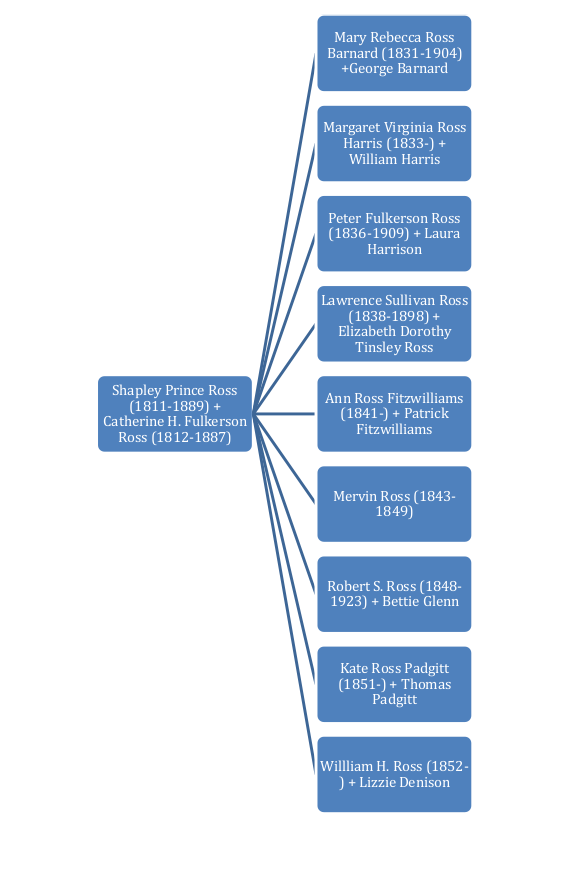
\includegraphics[width=0.6\linewidth]{figures/shapley_ross_family_tree}
\caption{Shapley Ross family tree. Taken without permission from \cite{rosspapersummary}.}
\end{figure}

\begin{figure}[h]
\centering
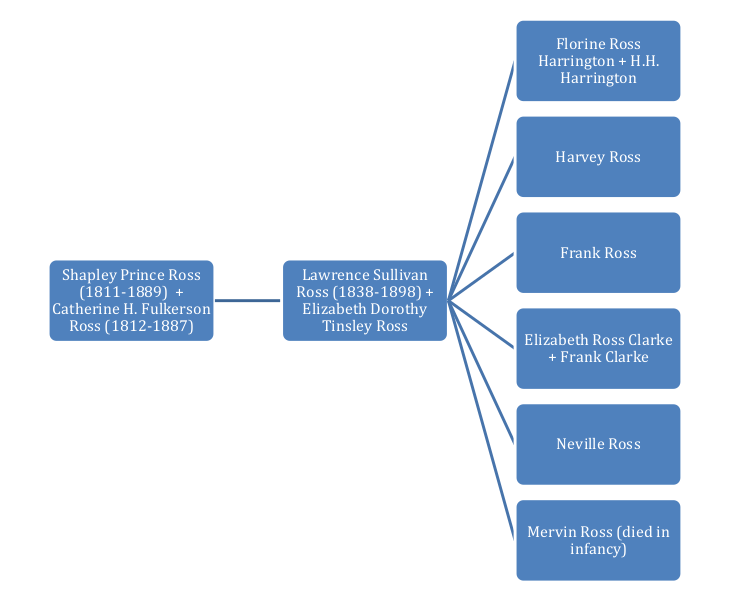
\includegraphics[width=0.7\linewidth]{figures/lawrence_ross_family_tree}
\caption{Lawrence Ross family tree. Taken without permission from \cite{rosspapersummary}.}
\end{figure}

% -----------------------------------------------------
% References.
% -----------------------------------------------------
\newpage
\section{end}

\newpage
\printbibliography

% -----------------------------------------------------
% End document.
% -----------------------------------------------------
\end{document}







